
\section*{Two atom simulations 2a)}
\subsection*{i}
\textbf{Write a function which solves equation (3) for two atoms and finds the positions and velocities
of the atoms as a function of time. Implement three different integration methods: Euler,
Euler-Cromer and Velocity-Verlet (see appendix C on page 11 for a description of the latter)}
We have created the Euler, EulerCromer and Velocity verlet algorithms. See appendix A for the kode. 

\section*{2b)}

\subsection*{2b) i)}
\textbf{. Simulate the motion of two atoms which start at rest separated by a distance of $1.5\sigma$ Use $\delta t  = 0.01$, simulate until $t
0 = 5$ and integrate with the Euler-Cromer method.}

\subsection*{2b) ii)}
\textbf{Plot the distance between the atoms as a function of time.}
We place two particles, one at origo and the other at positon  $(1.5\sigma, 0, 0)$. We therefore expect motion to be only happening on the x-axis. Using $\delta t$ of $0.01$, for $T = 5$. We simulate using Euler Cromer.

We plot the distance between the two particles in Figure (\ref{fig:two-particle-distance-15}).
\begin{figure}[h!]
        \centering 
        %Scale angir størrelsen på bildet. Bildefilen må ligge i samme mappe som tex-filen. 
        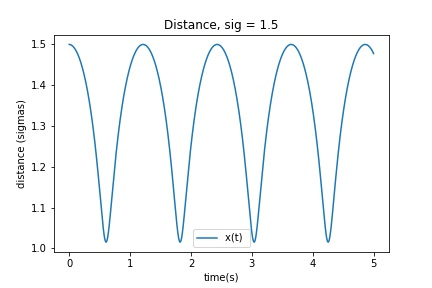
\includegraphics[scale=0.8]{./py/two-particle-distance-15.jpg} 
        \caption{Argon distance  with $D = 1.5 \sigma, \epsilon = 1$ and $\sigma = 1$, }
        %Label gjør det enkelt å referere til ulike bilder.
        \label{fig:two-particle-distance-15}
\end{figure}

\subsection*{2b) iii)}
\textbf{How does the motion fit with your expectations from exercise 1a) on the preceding page?}
Due to the potential not being symmetric, the expectation was that the particles would move more slowly toward each other than apart. We can see that the particles are being pulled toward each other constantly. 

\subsection*{iv)}
\textbf{Repeat the previous tasks, but now with an initial separation of $0.95 \sigma$. Explain your results}
In this second experiment, the two atoms are positioned closer, and within the region where the repulsive force dominates. Figure  (\ref{fig:two-particle-distance-095} shows how their distance increases rapidly. Because the repulsive energy is so much stronger than the attractive, a distance of $0.95\sigma$ we re in the repulsive range of the Lennard Jones potential. This accellerates the particles away from each other strongly enough that the particles eventually escape the attraction between particles and continue in opposite direcitons. 

\begin{figure}[h!]
        \centering 
        %Scale angir størrelsen på bildet. Bildefilen må ligge i samme mappe som tex-filen. 
        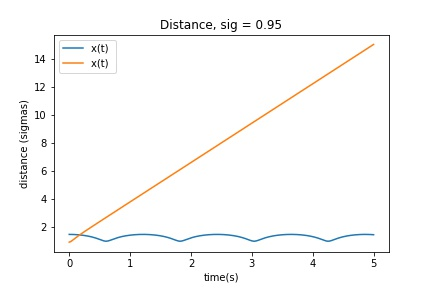
\includegraphics[scale=0.8]{./py/two-particle-distance-095.jpg} 
        \caption{Argon distance with $D = 0.95 \sigma, \epsilon = 1$ and $\sigma = 1$ }
        %Label gjør det enkelt å referere til ulike bilder.
        \label{fig:two-particle-distance-095}
\end{figure}


\newpage
\section*{2c}


\subsection*{2c) i)}
 \textbf{Plot the kinetic, potential and total energy as a function of time for the two cases in the previous
section}

Plotting the total energy in Figure \ref{fig:allEnergies}.

\begin{figure}[h!]
        \centering 
        %Scale angir størrelsen på bildet. Bildefilen må ligge i samme mappe som tex-filen. 
        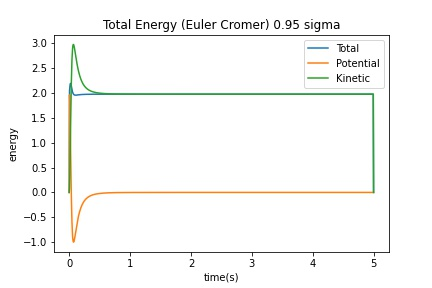
\includegraphics[scale=0.8]{./py/2ci_allEnergiesCromer15.jpg} 
        \caption{Euler Cromer method : Argon distance with $D = 1.5 \sigma, \epsilon = 1$ and $\sigma = 1$ }
        %Label gjør det enkelt å referere til ulike bilder.
        \label{fig:allEnergiesEuler15}
\end{figure}


\begin{figure}[h!]
        \centering 
        %Scale angir størrelsen på bildet. Bildefilen må ligge i samme mappe som tex-filen. 
        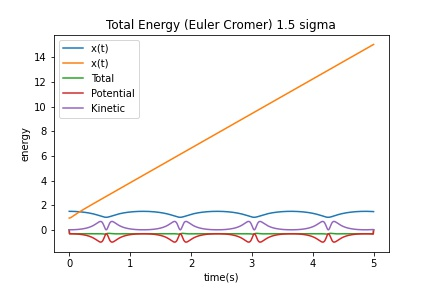
\includegraphics[scale=0.8]{./py/2ci_allEnergiesCromer095.jpg} 
        \caption{Euler cromer method : Argon distance with $D = 0.95 \sigma, \epsilon = 1$ and $\sigma = 1$ }
        %Label gjør det enkelt å referere til ulike bilder.
        \label{fig:allEnergiesEuler95}
\end{figure}


\subsection*{2c ) ii)}
\textbf{Theoretically speaking, should the total energy be conserved? Why, or why not? What about
momentum?
}

In theory, the energy should be conserved. Whenever two particles get into contact with each other, they will affect each other in a similar amount, but in opposite directions. As a result, kinetic energy will be conserved. As the potential energy is 0 when they are far away, there is no force acting on the particles.


\subsection*{2c ) iii)}
\textbf{How does the motion fit with your expectations from exercise 1a) on the preceding page?}
It fits exactly. Judging from the graphs, total energy is conserved in all the methods. . Kinetic energy is the velocity vector multiplied by the mass, potential energy is the sum of the acceleration force. TODO (What is potential energy, and is the kinetic energy really velocity vector multiplied by mass constant? What about sigma?


\subsection*{2c iv)}
\textbf{Simulate the same system as in exercise 2b) on the previous page with the Euler, Euler-Cromer
and Velocity Verlet algorithms, and compare graphs of the total energy as a function of time.}


When looking at figures \ref{fig:allEnergiesEuler15} to \ref{fig:allEnergiesVerlet95}, we see that the three methods have quite different charts for total energy. Velocity Verlet stabilizes at energy 5.6, Euler Cromer around 4.3 and Euler close to 6 in total Energy. It's unclear why there is such a large difference in integration methods. The fact that the total energy stabilizes indicates that there is no energy leak. Ideally, the blue line (total energy) should be flat.

\begin{figure}[h!]
        \centering 
        %Scale angir størrelsen på bildet. Bildefilen må ligge i samme mappe som tex-filen. 
        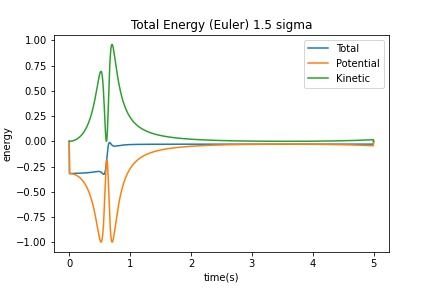
\includegraphics[scale=0.8]{./py/2civ_allEnergiesEuler15.jpg} 
        \caption{Euler method : Argon distance with $D = 1.5 \sigma, \epsilon = 1$ and $\sigma = 1$ }
        %Label gjør det enkelt å referere til ulike bilder.
        \label{fig:allEnergiesEuler15}
\end{figure}

\begin{figure}[h!]
        \centering 
        %Scale angir størrelsen på bildet. Bildefilen må ligge i samme mappe som tex-filen. 
        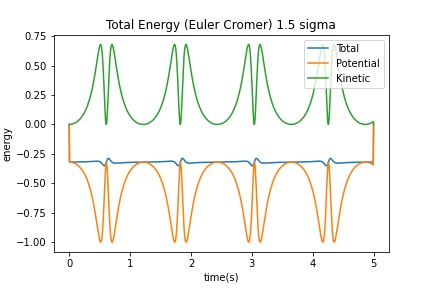
\includegraphics[scale=0.8]{./py/2civ_allEnergiesEulerCromer15.jpg} 
        \caption{Euler method : Argon distance with $D = 1.5 \sigma, \epsilon = 1$ and $\sigma = 1$ }
        %Label gjør det enkelt å referere til ulike bilder.
        \label{fig:allEnergiesEulerCromer15}
\end{figure}
\begin{figure}[h!]
        \centering 
        %Scale angir størrelsen på bildet. Bildefilen må ligge i samme mappe som tex-filen. 
        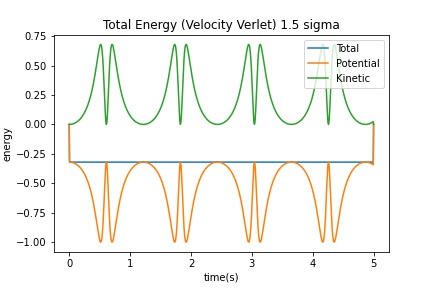
\includegraphics[scale=0.8]{./py/2civ_allEnergiesVelocityVerlet15.jpg} 
        \caption{Euler method : Argon distance with $D = 1.5 \sigma, \epsilon = 1$ and $\sigma = 1$ }
        %Label gjør det enkelt å referere til ulike bilder.
        \label{fig:allEnergiesVelver15}
\end{figure}

\begin{figure}[h!]
        \centering 
        %Scale angir størrelsen på bildet. Bildefilen må ligge i samme mappe som tex-filen. 
        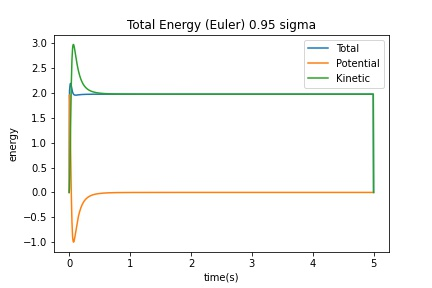
\includegraphics[scale=0.8]{./py/2civ_allEnergiesEuler095.jpg} 
        \caption{Euler  method : Argon distance with $D = 0.95 \sigma, \epsilon = 1$ and $\sigma = 1$ }
        %Label gjør det enkelt å referere til ulike bilder.
        \label{fig:allEuler95}
\end{figure}


\begin{figure}[h!]
        \centering 
        %Scale angir størrelsen på bildet. Bildefilen må ligge i samme mappe som tex-filen. 
        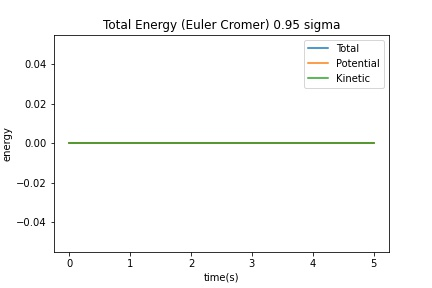
\includegraphics[scale=0.8]{./py/2civ_allEnergiesEulerCromer095.jpg} 
        \caption{Euler Cromer  method : Argon distance with $D = 0.95 \sigma, \epsilon = 1$ and $\sigma = 1$ }
        %Label gjør det enkelt å referere til ulike bilder.
        \label{fig:allEulerCromer95}
\end{figure}


\begin{figure}[h!]
        \centering 
        %Scale angir størrelsen på bildet. Bildefilen må ligge i samme mappe som tex-filen. 
        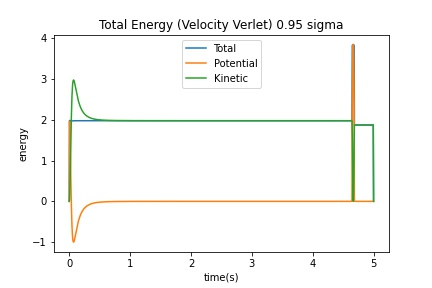
\includegraphics[scale=0.8]{./py/2civ_allEnergiesVelocityVerlet095.jpg} 
        \caption{Velocity verlet  method : Argon distance with $D = 0.95 \sigma, \epsilon = 1$ and $\sigma = 1$ }
        %Label gjør det enkelt å referere til ulike bilder.
        \label{fig:allEnergiesVerlet95}
\end{figure}





\subsection*{2c) v)}
\textbf{Find the largest time step that keeps stable motion and conserves energy for all three methods
(small fluctuations in energy are allowed as long as they are periodic and don’t increase/decrease
with time). Discuss your results.
}

When we experiment, we see that at a delta of $0.1$, the accuracy allows the particles to tunnel through each other to the other side. At half this, the graphs look pretty much the same except they are more pointy. With such low resolution graphs, it can be expected to be enough inaccuracy so that the simulation can be wrong.
The EulerCromer and Velocity Verlet are more resistant to higher delta t.

\subsection*{2c) vi)}
\textbf{Link your experimentation to a brief discussion of the pros and cons of the three methods, both
physically and computationally}

What method is a question of simplicity, accuracy and computational cost the $\delta t$.  The higher computational cost, the more accuracy is required for the algorithm to be viable. By including the second derivative, such as the acceleration, the Velocity Verlet approximates the change in the velocity using - basically - a second order Taylor polynomial. This additional complexity inside the algorithm, allowing it to "look ahead" and predict changes to the acceleration and velocity, allows a significantly longer $\delta t$. This might be enough to defend the computational cost of adding more terms, and so the algorithm might emerge faster on average.

However, the more complex an algorithm is, the more difficult it is to write and understand, and debug. If an agorithm is 10\% more effective, and takes 10 more hours to write and debug, the algorithm must run for at least 100 hours to recoup the loss on a machine with the same cost-basis as the developer. Usually, computing speed is less expensive than developer time, so its often much worse.

\subsection*{2d) i}
\textbf{. Extend your implementation such that it writes to an xyz-file at each timestep (see appendix A on page 11).}

The implementation writes to an xyz file, which can be opened by Ovito.

\subsection*{2d) ii}
\textbf{Visualise the results of your simulations using Ovito (see appendix B on page 11)}


\begin{figure}[h!]
        \centering 
        %Scale angir størrelsen på bildet. Bildefilen må ligge i samme mappe som tex-filen. 
        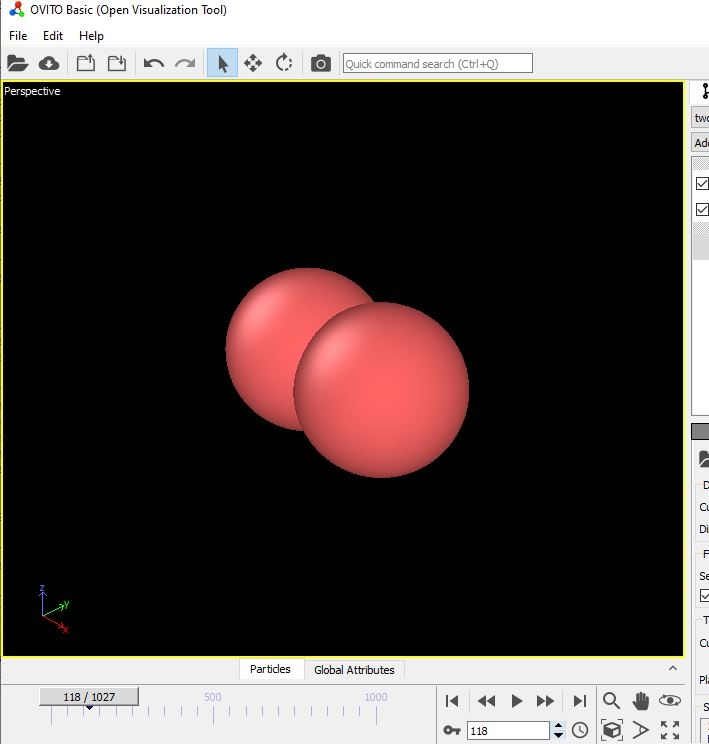
\includegraphics[scale=0.6]{./py/2dii_ovito.JPG} 
        \caption{Two atoms at distance $1.5 \sigma $ visualized in Ovito }
        %Label gjør det enkelt å referere til ulike bilder.
        \label{fig:2dii_ovito}
\end{figure}
